% !TEX root = main.tex
% !TEX root = main.tex
\documentclass[letterpaper, 11pt]{extarticle}
% \usepackage{fontspec}

% ==================================================

% document parameters
% \usepackage[spanish, mexico, es-lcroman]{babel}
\usepackage[english]{babel}
\usepackage[margin = 1in]{geometry}

% ==================================================

% Packages for math
\usepackage{mathrsfs}
\usepackage{amsfonts}
\usepackage{amsmath}
\usepackage{amsthm}
\usepackage{amssymb}
\usepackage{physics}
\usepackage{dsfont}
\usepackage{esint}

% ==================================================

% Packages for writing
\usepackage{enumerate}
\usepackage[shortlabels]{enumitem}
\usepackage{framed}
\usepackage{csquotes}

% ==================================================

% Miscellaneous packages
\usepackage{float}
\usepackage{tabularx}
\usepackage{xcolor}
\usepackage{multicol}
\usepackage{subcaption}
\usepackage{caption}
\captionsetup{format = hang, margin = 10pt, font = small, labelfont = bf}

% Citation
\usepackage[round, authoryear]{natbib}

% Hyperlinks setup
\usepackage{hyperref}
\definecolor{links}{rgb}{0.36,0.54,0.66}
\hypersetup{
   colorlinks = true,
    linkcolor = black,
     urlcolor = blue,
    citecolor = blue,
    filecolor = blue,
    pdfauthor = {Author},
     pdftitle = {Title},
   pdfsubject = {subject},
  pdfkeywords = {one, two},
  pdfproducer = {LaTeX},
   pdfcreator = {pdfLaTeX},
   }

% \begin{document}
% Hello, world! This is a minimal document to test the preamble.
% \end{document}

\usepackage{listings} 
\usepackage{xcolor}

\definecolor{codegreen}{rgb}{0.12,0.6,0.33}
\definecolor{codegray}{rgb}{0.5,0.5,0.5}
\definecolor{codepurple}{rgb}{0.58,0,0.82}
\definecolor{codeblue}{rgb}{0,0.1,0.8}
\definecolor{backcolour}{rgb}{0.95,0.95,0.92}

\lstdefinestyle{pythonstyle}{
   backgroundcolor=\color{backcolour},
   commentstyle=\color{codegreen},
   keywordstyle=\color{codeblue}\bfseries,
   numberstyle=\tiny\color{codegray},
   stringstyle=\color{codepurple},
   basicstyle=\ttfamily\footnotesize,
   breakatwhitespace=false,
   breaklines=true,
   captionpos=b,
   keepspaces=true,
   numbers=left,
   numbersep=5pt,
   showspaces=false,
   showstringspaces=false,
   showtabs=false,
   tabsize=4,
   language=Python
}

% \usepackage{minted}

\usepackage{titlesec}
\usepackage[many]{tcolorbox}

% Adjust spacing after the chapter title
\titlespacing*{\chapter}{0cm}{-2.0cm}{0.50cm}
\titlespacing*{\section}{0cm}{0.50cm}{0.25cm}

% Indent 
\setlength{\parindent}{0pt}
\setlength{\parskip}{1ex}

% --- Theorems, lemma, corollary, postulate, definition ---
% \numberwithin{equation}{section}

\newtcbtheorem[]{problem}{Problem}%
    {enhanced,
    colback = black!5, %white,
    colbacktitle = black!5,
    coltitle = black,
    boxrule = 0pt,
    frame hidden,
    borderline west = {0.5mm}{0.0mm}{black},
    fonttitle = \bfseries\sffamily,
    breakable,
    before skip = 3ex,
    after skip = 3ex
}{problem}

\tcbuselibrary{skins, breakable}

% --- You can define your own color box. Just copy the previous \newtcbtheorm definition and use the colors of yout liking and the title you want to use.
% --- Basic commands ---
%   Euler's constant
\newcommand{\eu}{\mathrm{e}}

%   Imaginary unit
\newcommand{\im}{\mathrm{i}}

%   Sexagesimal degree symbol
\newcommand{\grado}{\,^{\circ}}

% --- Comandos para álgebra lineal ---
% Matrix transpose
\newcommand{\transpose}[1]{{#1}^{\mathsf{T}}}

%%% Comandos para cálculo
%   Definite integral from -\infty to +\infty
\newcommand{\Int}{\int\limits_{-\infty}^{\infty}}

%   Indefinite integral
\newcommand{\rint}[2]{\int{#1}\dd{#2}}

%  Definite integral
\newcommand{\Rint}[4]{\int\limits_{#1}^{#2}{#3}\dd{#4}}

%   Dot product symbol (use the command \bigcdot)
\makeatletter
\newcommand*\bigcdot{\mathpalette\bigcdot@{.5}}
\newcommand*\bigcdot@[2]{\mathbin{\vcenter{\hbox{\scalebox{#2}{$\m@th#1\bullet$}}}}}
\makeatother

%   Hamiltonian
\newcommand{\Ham}{\hat{\mathcal{H}}}

%   Trace
\renewcommand{\Tr}{\mathrm{Tr}}

% Christoffel symbol of the second kind
\newcommand{\christoffelsecond}[4]{\dfrac{1}{2}g^{#3 #4}(\partial_{#1} g_{#2 #4} + \partial_{#2} g_{#1 #4} - \partial_{#4} g_{#1 #2})}

% Riemann curvature tensor
\newcommand{\riemanncurvature}[5]{\partial_{#3} \Gamma_{#4 #2}^{#1} - \partial_{#4} \Gamma_{#3 #2}^{#1} + \Gamma_{#3 #5}^{#1} \Gamma_{#4 #2}^{#5} - \Gamma_{#4 #5}^{#1} \Gamma_{#3 #2}^{#5}}

% Covariant Riemann curvature tensor
\newcommand{\covariantriemanncurvature}[5]{g_{#1 #5} R^{#5}{}_{#2 #3 #4}}

% Ricci tensor
\newcommand{\riccitensor}[5]{g_{#1 #5} R^{#5}{}_{#2 #3 #4}}

\begin{document}

\textsf{\LARGE{\textbf{Take-home exam 3}}}

\normalsize{\textit{Dynamical Systems}}

\vspace{1ex}

\textsf{\textbf{Student:}} \text{Males-Araujo Yorlan}, 
\href{mailto:yorlan.males@yachaytech.edu.ec}{\texttt{yorlan.males@yachaytech.edu.ec}}\\
\textsf{\textbf{Lecturer:}} \text{Cosenza Mario}, 
\href{mcosenza@yachaytech.edu.ec}{\texttt{mcosenza@yachaytech.edu.ec}}

Yachay Tech, \today.

\vspace{2ex}

\begin{problem}{Bifurcation diagram and Lyapunov exponent}{problem-label-2}

Consider the following map $f(x_n) \in [0, 1]$,
\[
x_{n+1} = f(x_n) = x_n +\omega -\frac{1}{2\pi}\sin(2\pi x_n) \text{ mod } 1.
\]

\begin{enumerate}[(a)]
    \item Plot the bifurcation diagram of $x_n$ vesurs $\omega$. [1]
    \item Calculate the Lyapunov exponent as a function of $\omega$. [1]
\end{enumerate}
\end{problem}

\begin{enumerate}[(a)]
    \item Reusing code from the previous exam, we obtained the bifurcation diagram for $\omega \in [0, 2]$.
    \begin{figure}[!ht]
        \centering
        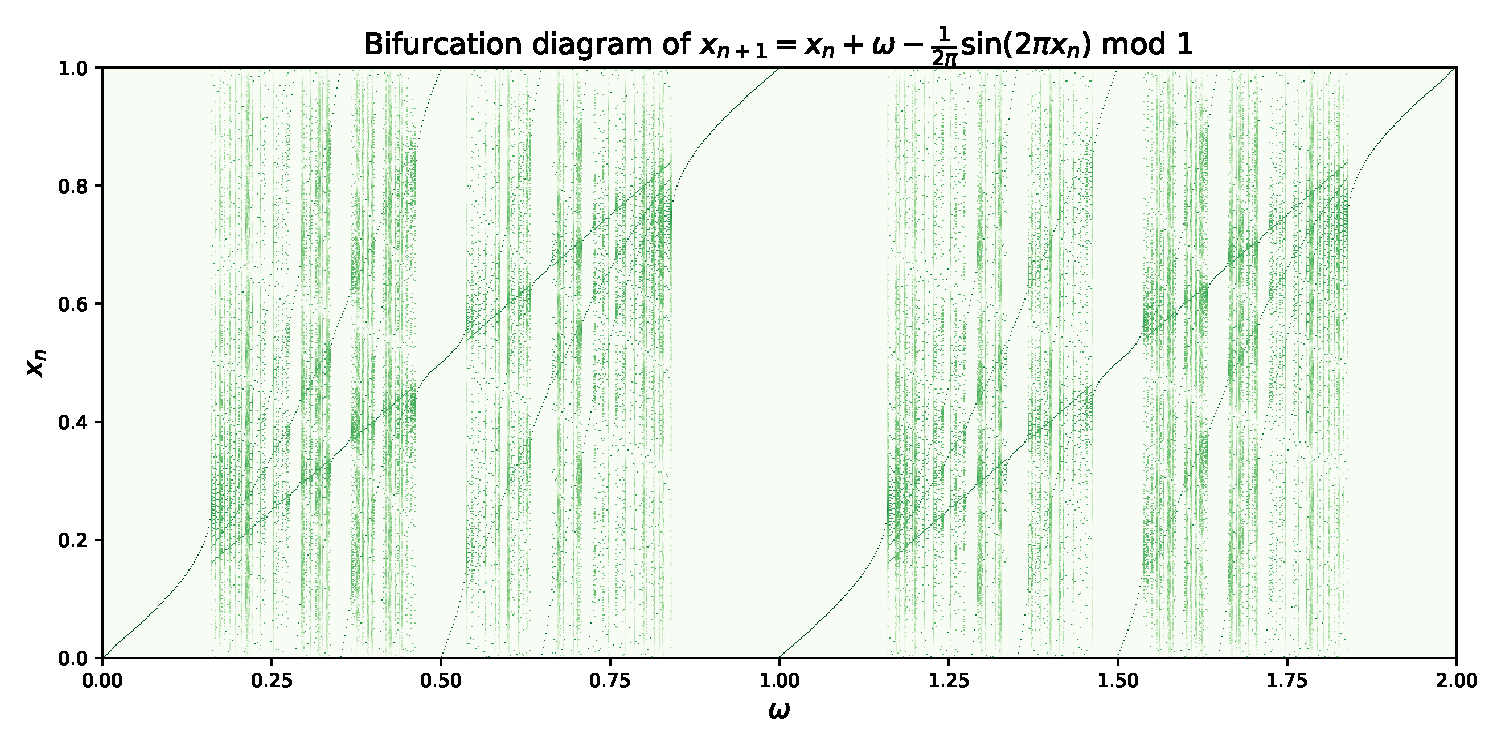
\includegraphics[scale=0.60]{images/CIRCLE-GREENS.pdf}
        \caption{Long term behavior of the map $f(x_n)$ as a function of $\omega$.}
        \label{fig:1a}
    \end{figure}

    We observe the diagram repeats itself after $\omega = 1$.

    \item Again, recycling code, we calculated the Lyapunov exponent as a function of $\omega$, and 
    we show the figure below.
    \begin{figure}[!ht]
        \centering
        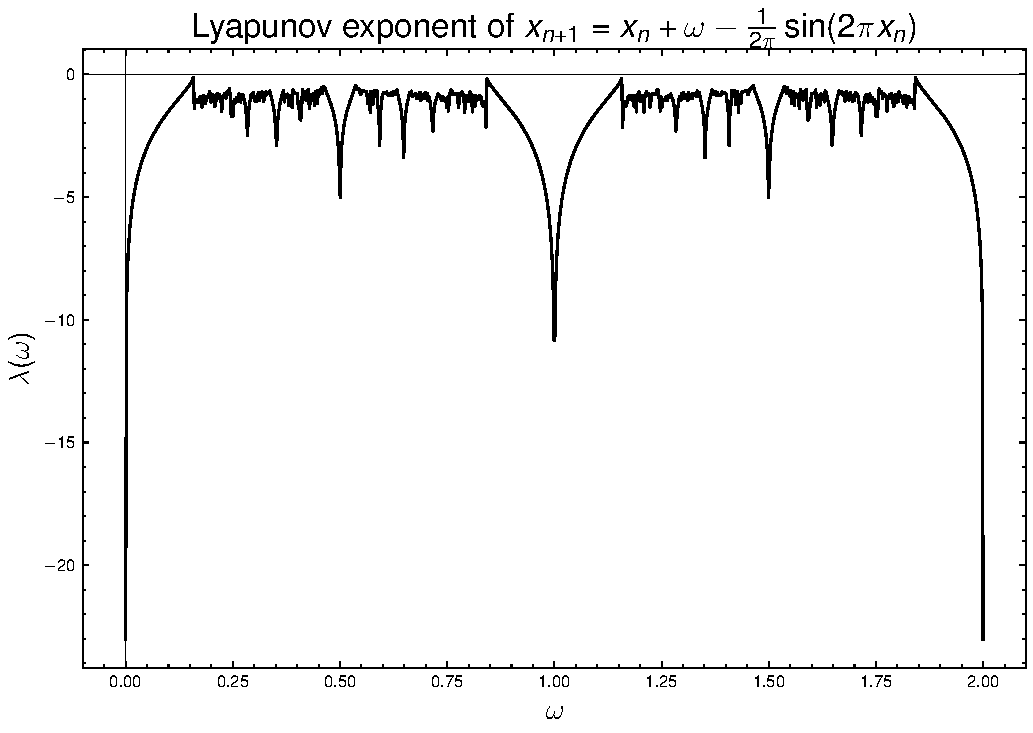
\includegraphics[scale=0.65]{images/cir_lya.pdf}
        \caption{Behavior of the map as a function of $\omega$.}
        \label{fig:1b}
    \end{figure}

    \newpage
    It seems to match with the bifurcation diagram. Moreover, it appears to be 
    negative for the most part of the interval, except at some points where it is equal to zero.
    This indicates that the map is mostly stable.
\end{enumerate}

\begin{problem}{Two-dimensional map analysis}{problem-label-3}

Consider the two-dimensional map
\begin{align*}
    x_{n+1} &= 1-a|x_n|+y_n, \\
    y_{n+1} &= bx_n
\end{align*}
where $a$ and $b$ are real parameters.

\begin{enumerate}[(a)]
    \item By using an initial condition close to the origin, plot the attractor
    for $a=1.7$ and $b=0.5$. Is is a strange attractor? [1]
    \item Plot the bifurcation diagram of $x_n$ as a function of $b \in [-0.7, 0.7]$,
    with fixed value $a=1.5$. [1]
    \item Calculate the Lyapunov exponents for this map as functions the parameters $a$ and $b$. [1]
    \item Calculate the fractal dimension of the the attractor for $a=1.7$ and $b=0.5$. [1] 
\end{enumerate}
\end{problem}

\begin{enumerate}[(a)]
    \item Setting functions for each variable (plugging $y_{n}$ in $x_{n+1}$), we plotted the attractor for the given parameters. Of course,
    we excluded the first iterations to avoid the transient behavior. The attractor is shown in Figure \ref{fig:2a}.
    \begin{figure}[!ht]
        \centering
        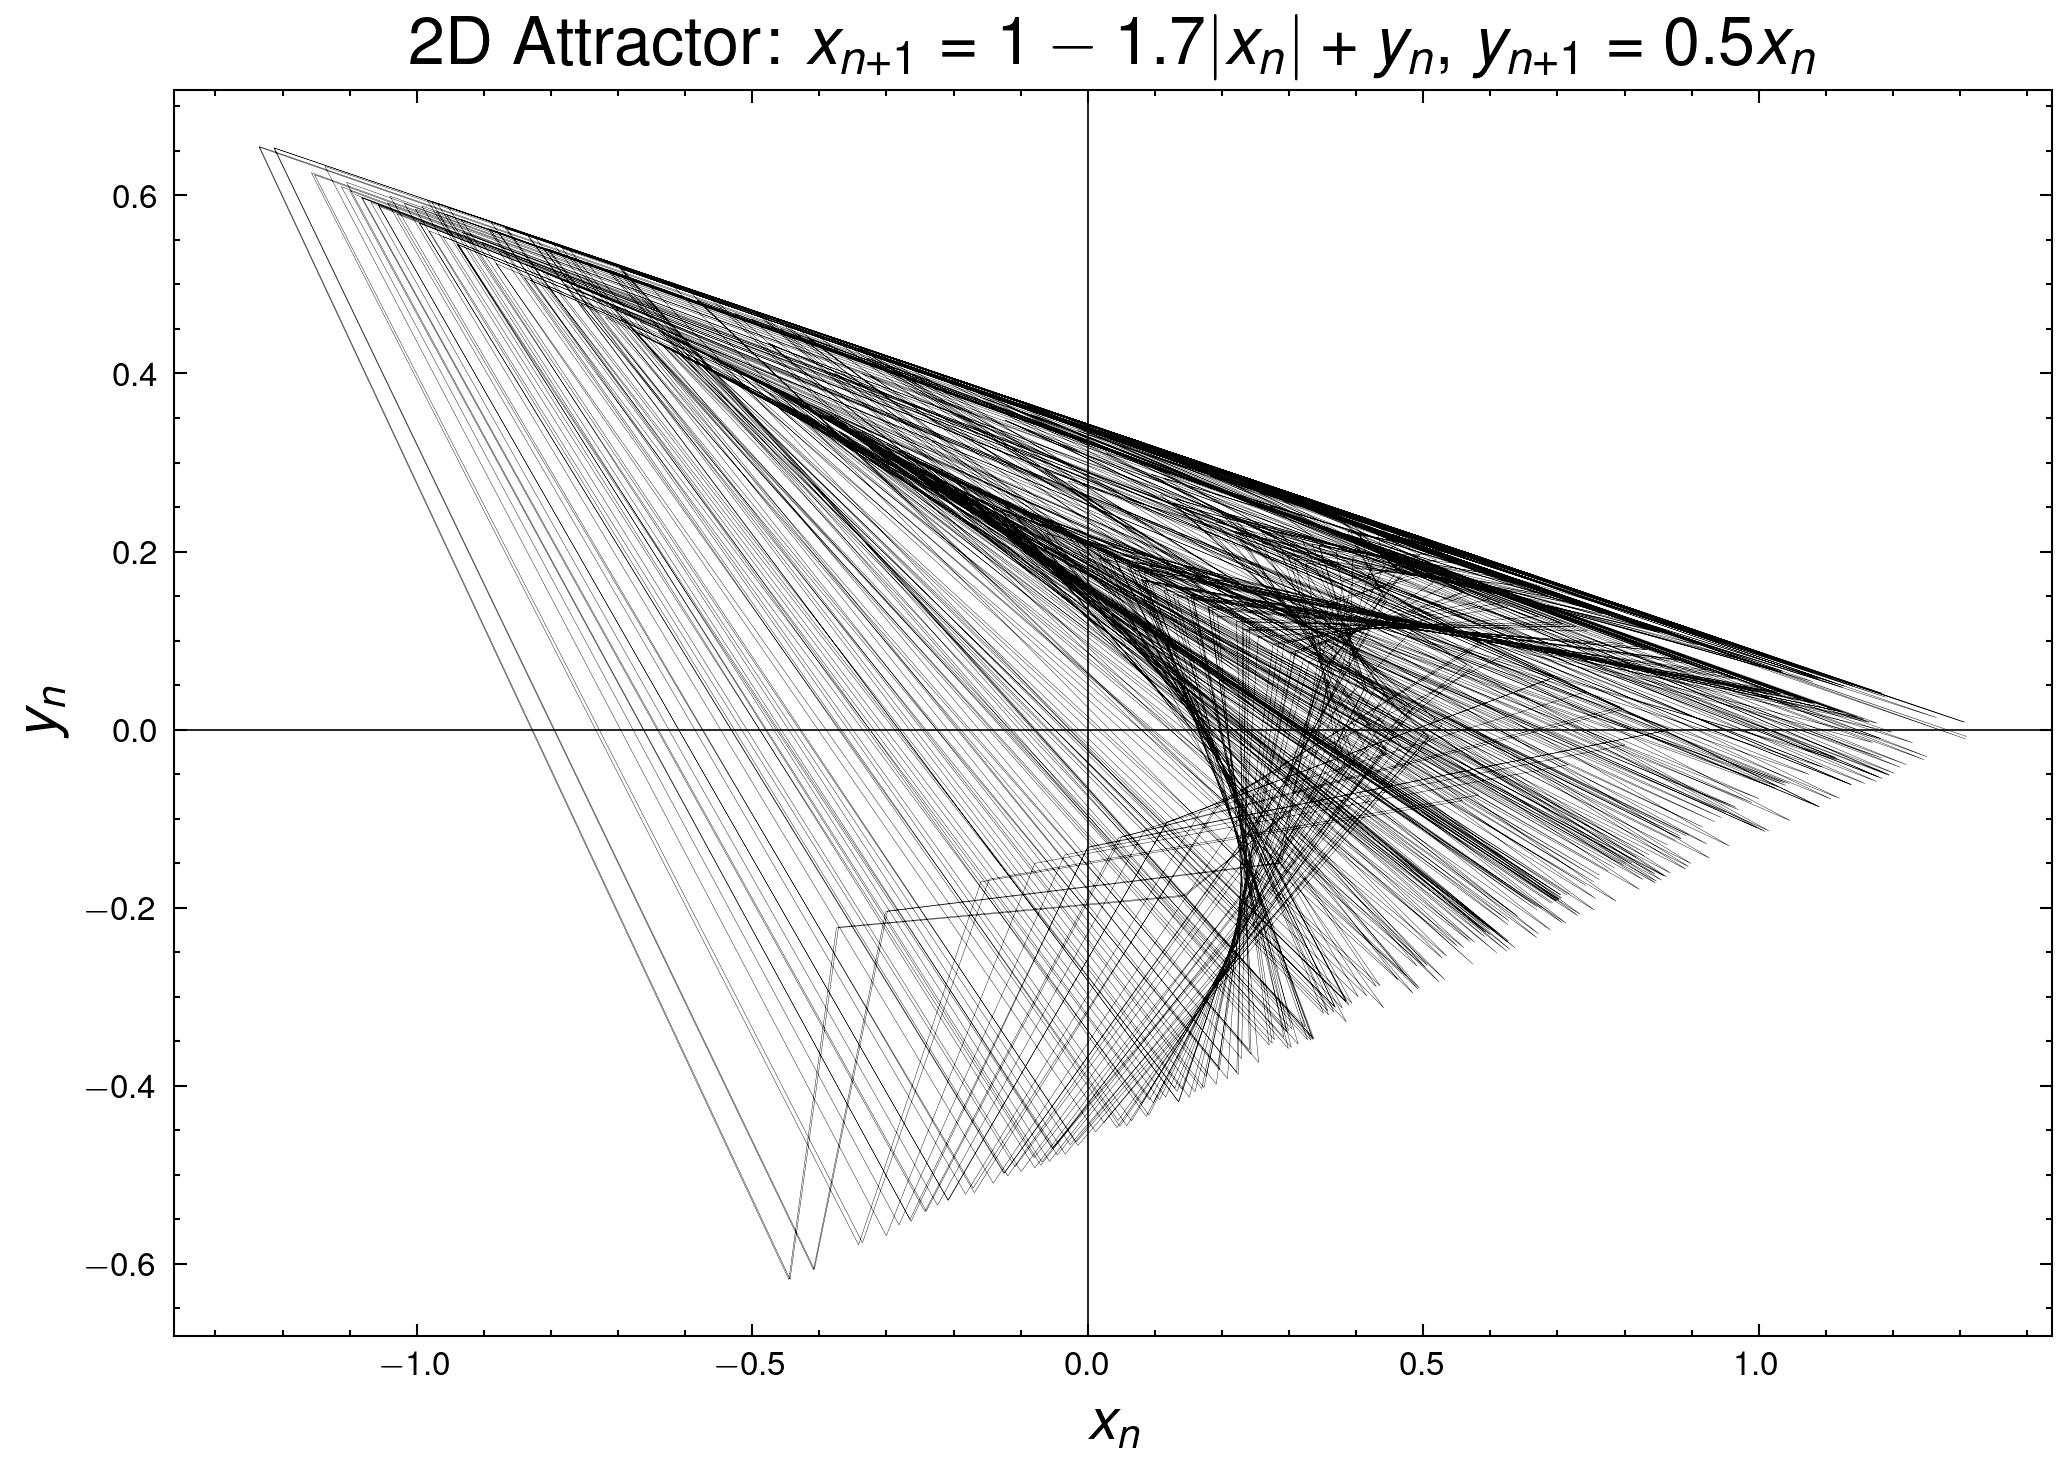
\includegraphics[scale=0.70]{images/two_dim_map.png}
        \caption{Attractor of the system for $a=1.7$ and $b=0.5$.}
        \label{fig:2a}
    \end{figure}

    \newpage
    We can see that the attractor is indeed strange and looks like a fractal. It's awesome.
    \item The results of the calculation is shown in Figure \ref{fig:2b}. It has a funny yet intriguing shape.
    
    \begin{figure}[!ht]
        \centering
        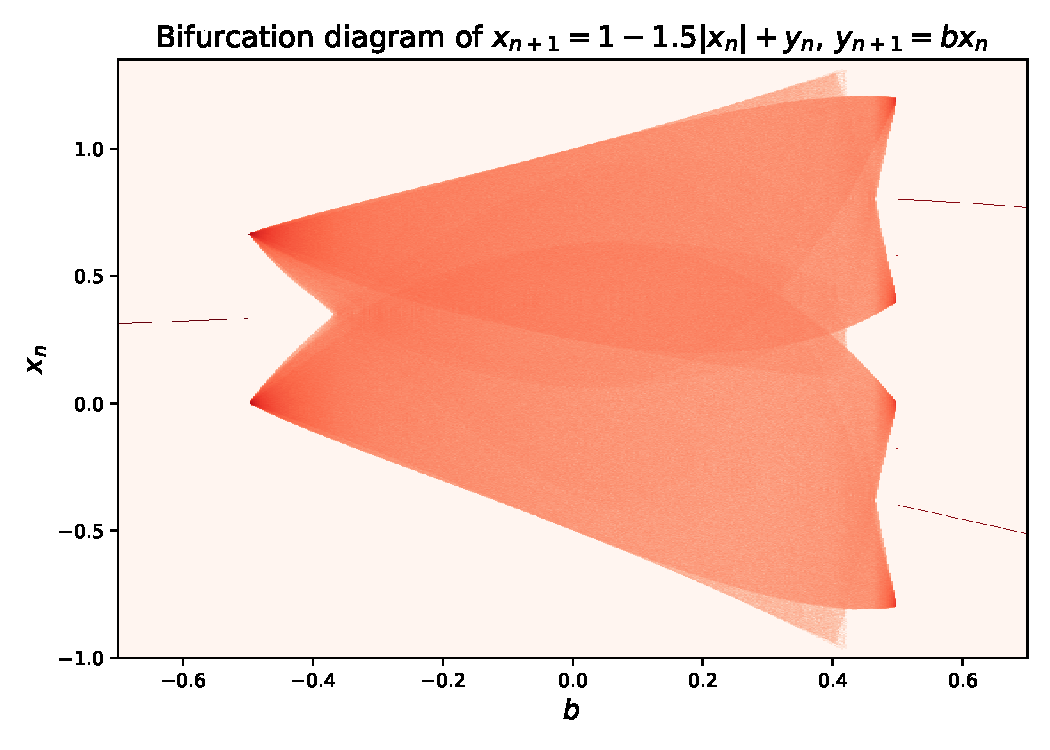
\includegraphics[scale=0.70]{images/TWO-MAP-REDS.pdf}
        \caption{Long term values of the map as a function of $b$ with fixed $a=1.5$.}
        \label{fig:2b}
    \end{figure}

    \item We calculated the Lyapunov exponent for both parameters $a$ and $b$,
    and plotted the results using a heatmap, where colors convey information about the 
    magnitude of the exponent. The results are shown in Figure \ref{fig:2c}.

    \begin{figure}[!ht]
        \centering
        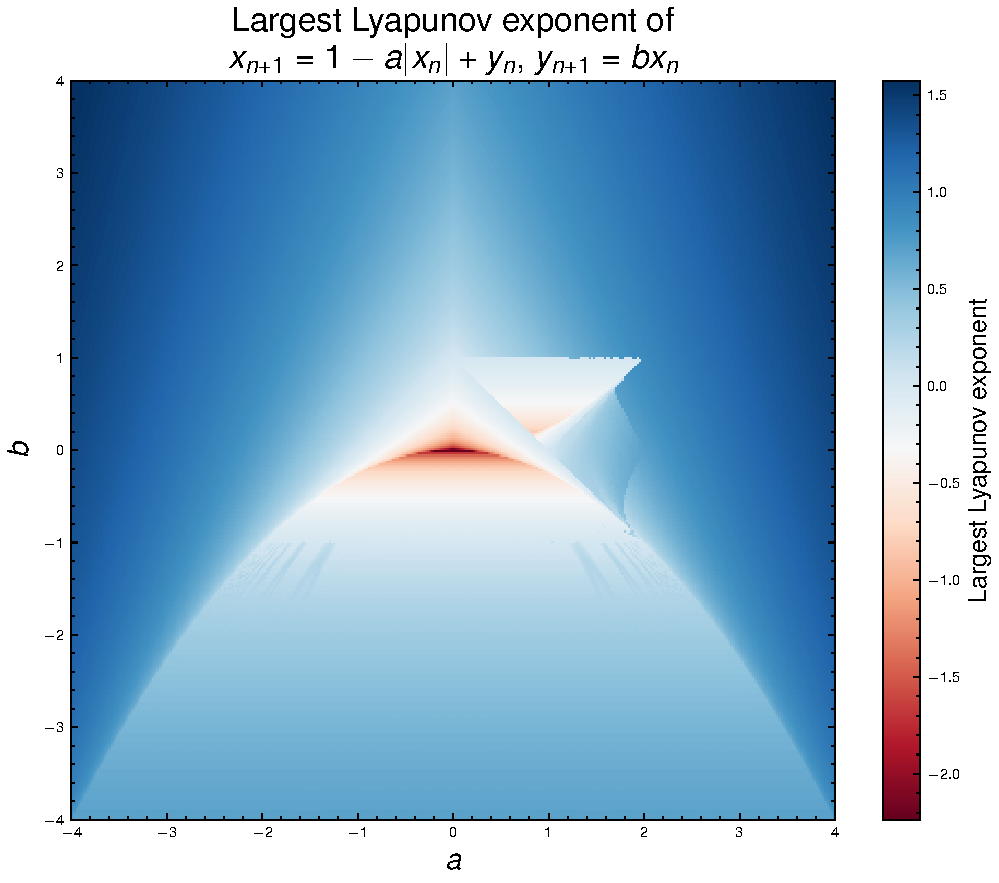
\includegraphics[scale=0.80]{images/lyapunov_2d.pdf}
        \caption{Lyapunov exponent heatmap of the two-dimensional map.}
        \label{fig:2c}
    \end{figure}

    We took, as reviewed in class, the largest Lyapunov exponent. The results are stunning;
    it seems to display some kind of structure. We can also see that it is mostly positive.

    \item To calculate the fractal dimension, we used the Kaplan-Yorke formula. Since the map
    contains an absolute value, we had to consider both cases: $x > 0$ and $x<0$. However, we found
    the same result for both cases, so we'll just show the case $x>0$.
    
    For $a=1.7$ and $b=0.5$, the Jacobian matrix is given by
    \[
    J = \begin{pmatrix}
        -1.7 & 1 \\
        0.5 & 0
    \end{pmatrix},
    \]
    so that the characteristic equation is
    \[
    \mu^2 + 1.7\mu - 0.5 = 0.
    \]
    The roots of this equation are
    \begin{align*}
        \mu_{1} & \approx 0.25567,\\
        \mu_{2} & \approx -1.95567.
    \end{align*}
    With these, we can obtain the Lyapunov exponents via $e^{\lambda} = \mu$. We have
    \begin{align*}
        \lambda_{1} & = \ln(0.25567) \approx -1.3638,\\
        \lambda_{2} & = \ln(-1.95567) \approx 0.6707,
    \end{align*}
    where we took the real part of the argument in the second logarithm.

    Since $\lambda_{1} < 0$ and $\lambda_{2} > 0$, the fractal dimension of the attractor 
    for the given parameters is
    \[
    \boxed{
        D_f = 1 + \frac{\lambda_2}{|\lambda_1|} = 1 + \frac{0.6707}{1.3638} \approx 1.49.
    }
    \]
\end{enumerate}

\begin{problem}{Escape and repeller}{problem-label-4}

Consider the map
\[
x_{n+1} = \frac{a}{2}\left(1-|1-2x_n|\right).
\]

\begin{enumerate}[(a)]
    \item Show that $x_n$ escapes the interval $[0,1]$ for $a=2+\epsilon$. [1]
    \item Calculate the fractal dimension of the repeller set as a function of $\epsilon$. [1]
\end{enumerate}

\end{problem}

\begin{enumerate}[(a)]
    \item This can be done by just iterating the map for $a=2+\epsilon$ and checking if the values of $x_n$
    escape the interval $[0,1]$. A result of this is shown in Figure \ref{fig:4a}.

    \begin{figure}[!ht]
        \centering
        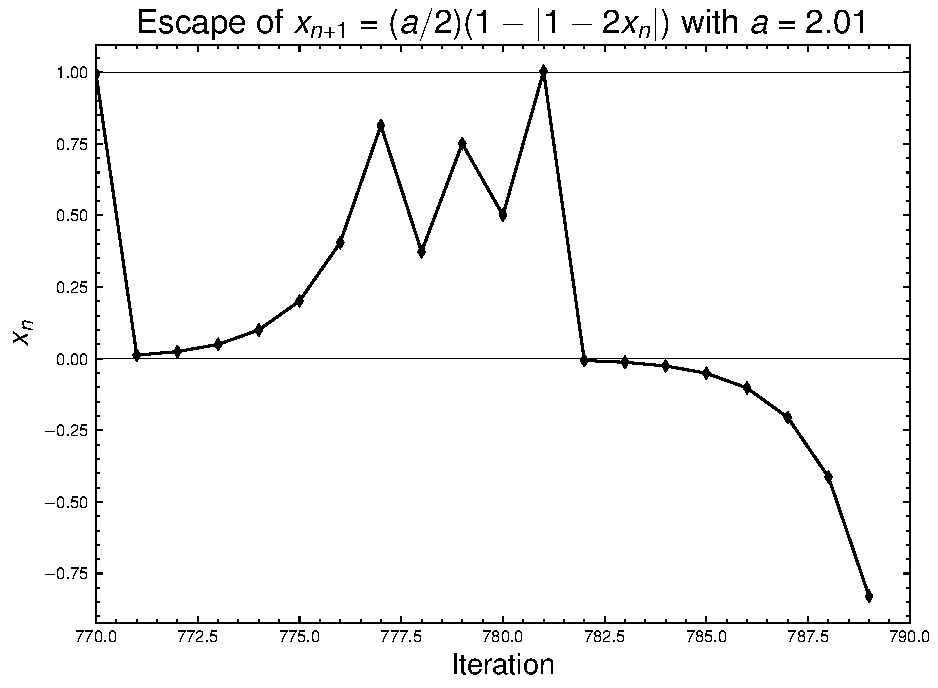
\includegraphics[scale=0.70]{images/escape_map.pdf}
        \caption{Escape of the map for $a=2+\epsilon$.}
        \label{fig:4a}
    \end{figure}

    The map does escape the interval if $a > 2$.
    \item The fractal dimension of the repeller set was calculated using the escape rate method. 
    For each value of $\epsilon$, we sampled initial points across $[0,1]$ and determined which points
    remained bounded after many iterations. The fractal dimension was then computed using the formula 
    \[
    D = 1 - \frac{\gamma}{\ln(a)}
    \]
    where $\gamma$ is the escape rate. We plot the fractal dimension as a function of $\epsilon$ in Figure \ref{fig:4b}.
    \begin{figure}[!ht]
        \centering
        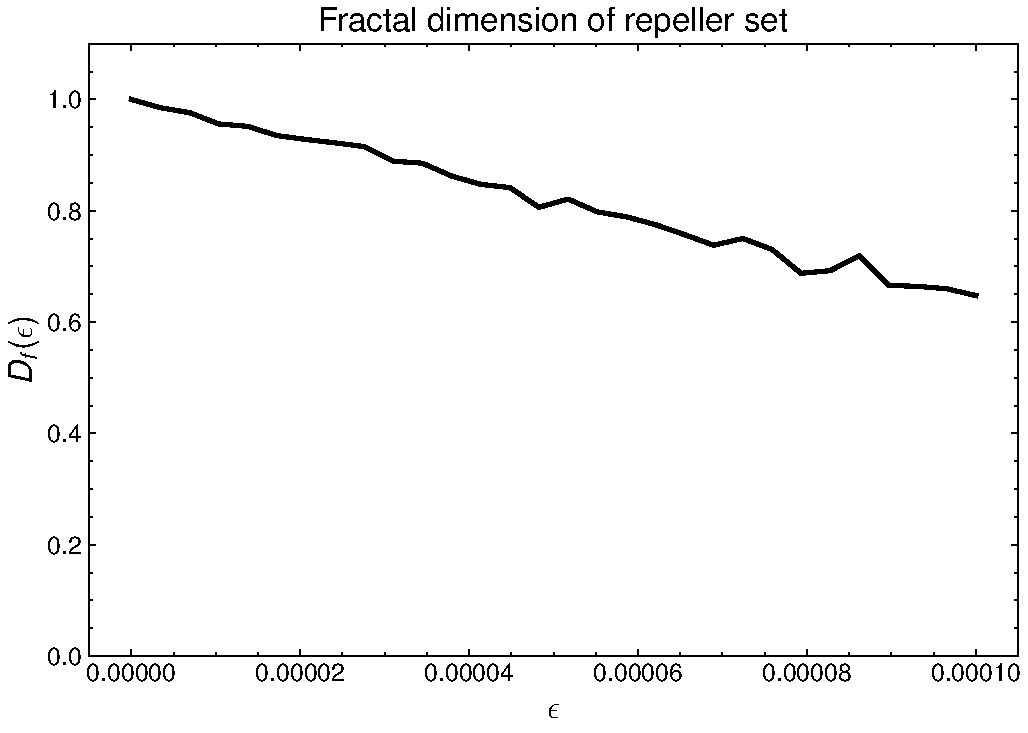
\includegraphics[scale=0.70]{images/fractal_dimension_repeller.pdf}
        \caption{Repeller's fractal dimension.}
        \label{fig:4b}
    \end{figure}

    The fractal dimension decreases as $\epsilon$ increases.
\end{enumerate}

\begin{problem}{GOY method}{problem-label-5}

The logarithmic map
\[
x_{n+1}=b+\ln|x_n|
\]
exhibits robuts chaos in the parameter interval $b \in [0,1]$.

\begin{enumerate}[(a)]
    \item Calculate the unstable fixed point for $b \in [0,1]$. [1]
    \item Use the GOY method for controlling chaos to stabilize the fixed point at $b=0$.
    Show the time series of $x_n$ before and after the control is applied. [1]
\end{enumerate}
\end{problem}

\begin{enumerate}[(a)]
    \item The fixed point is found by solving the equation
    \[
    x^*=\ln|x^*| \implies x^* - \ln|x^*| = 0.
    \]
    We did it numerically, and the result is shown below.

    \begin{figure}[!ht]
        \centering
        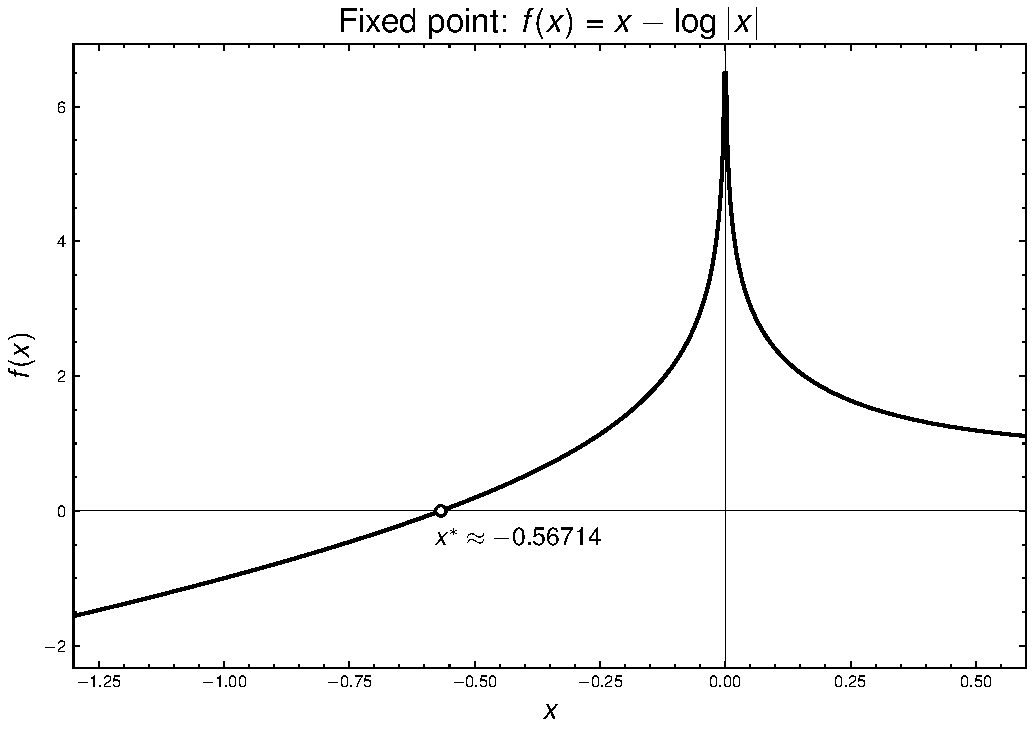
\includegraphics[scale=0.70]{images/fixed_point.pdf}
        \caption{Fixed point found.}
        \label{fig:4b}
    \end{figure}

    \newpage
    It was also found to be \textit{unstable} since the absolute value
    of the derivative evaluated at the point is less than $1$.

    \item Since the point is unstable, we can apply the GOY method. 
    
    First, to verify the point was actually unstable, we plotted the time series
    given some initial condition. This is shown in Figure \ref{fig:5ba}.

    \begin{figure}[!ht]
        \centering
        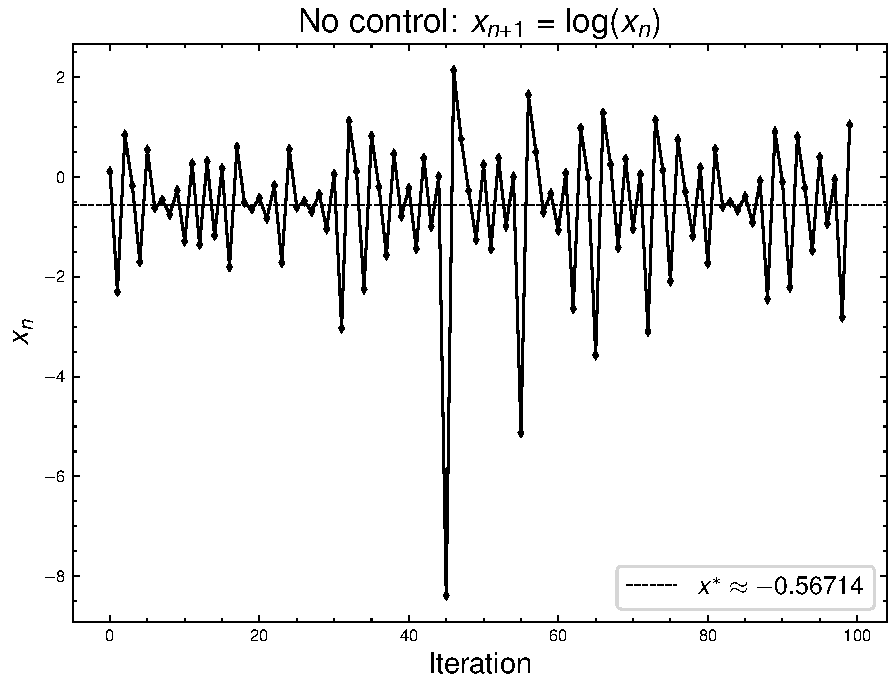
\includegraphics[scale=0.70]{images/no_control_log.pdf}
        \caption{Not controlled map.}
        \label{fig:5ba}
    \end{figure}

    We observe the evolution kind of oscillates around the unstable fixed point in short intervals.

    After doing that, we implemented the GOY method to keep the evolution close to the fixed
    point by providing small kicks when it tries to go further from it. By doing this,
    we were able to control chaos. The final results are shown below.

    \begin{figure}[!ht]
        \centering
        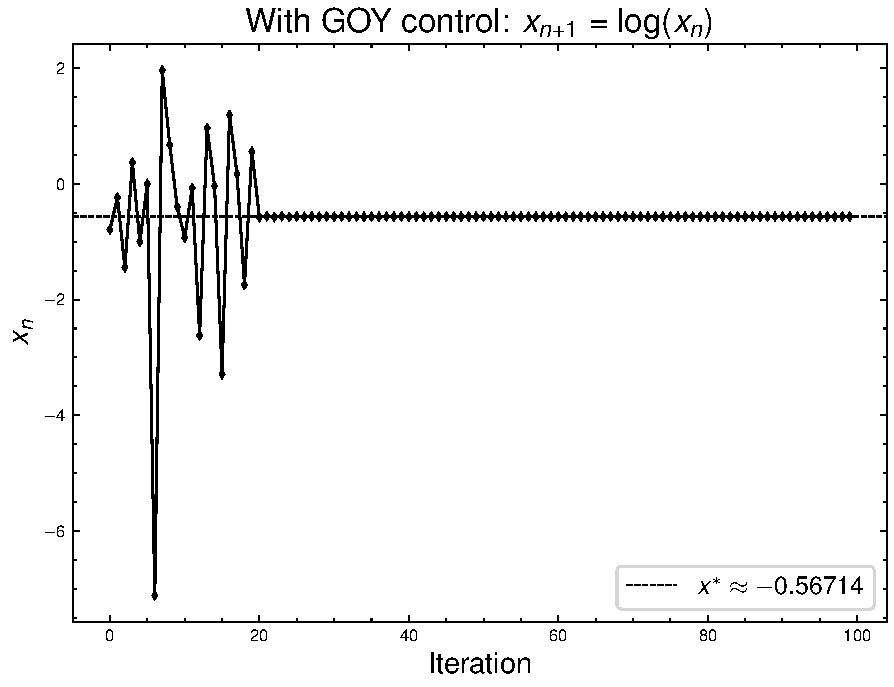
\includegraphics[scale=0.70]{images/goy_control.pdf}
        \caption{Chaos being controlled around the unstable fixed point.}
        \label{fig:4b}
    \end{figure}

    Once the map gets close to the point, the method switches on and it does let it leave. 
    It turned out to be great.

\end{enumerate}

Thank you for the course and everything, prof. Mario. Truly life-changing.

% \newpage
% \vspace{0.1ex}

% \bibliographystyle{apalike}
% \bibliography{references}

\end{document}